\chapter{Installation and First Steps: Double Link List}

\section{Step 01: Install Enterprise Architect}
$\blacktriangleright$ Download and install EA (Figure
\ref{fig_enterpriseArchitextHomepage})\\ 
Go to http://www.sparxsystems.com.au/ to get a free 30 day trial.\\
\begin{figure}[!h]
	\centering
  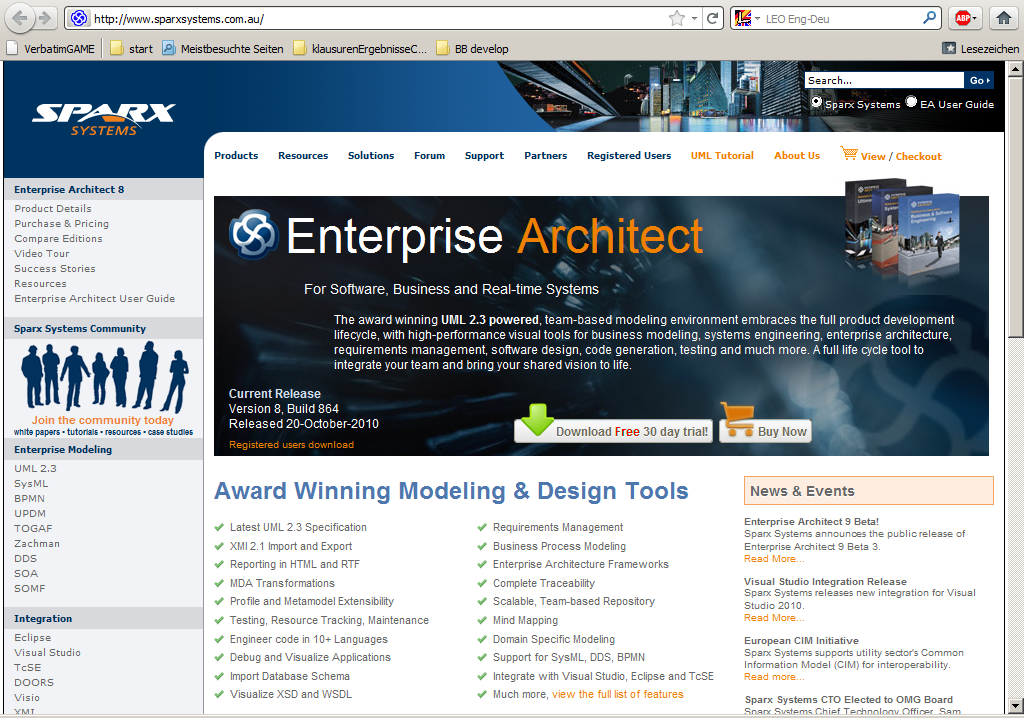
\includegraphics[width=0.5\textwidth]{pics/ea_download.png}
	\caption{Enterprise Architect Homepage}
	\label{fig_enterpriseArchitextHomepage}
\end{figure}

$\blacktriangleright$ Install our EA-Plugin (Figure \ref{fig_eaPluginWizard})\\
Go to
\url{http://www.moflon.org/fileadmin/download/moflon-ide/eclipse-plugin/ea-ecore-addin/ea-ecore-addin.zip}
Just unpack the ZIP-File, run setup.exe and follow the instructions.

\begin{figure}[!h]
	\centering
  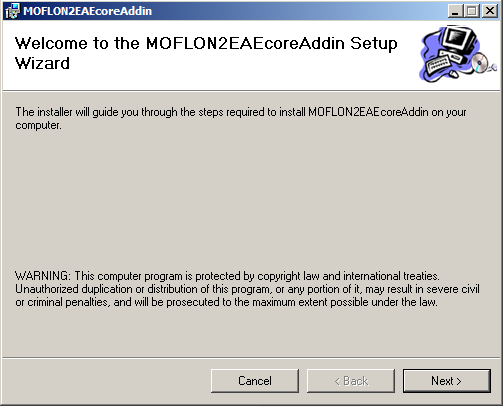
\includegraphics[width=0.3\textwidth]{pics/eaplugin_install.png}
	\caption{EA-Plugin Wizard}
	\label{fig_eaPluginWizard}
\end{figure}

\section{Step 02: Install Eclipse}
$\blacktriangleright$ Install the latest version of JAVA (JDK).\\ %WO? bild ?
%URL! online tutorial

$\blacktriangleright$ Download the modeling Package ``Eclipse Modeling Tools
(includes Incubating components)'' (Figure \ref{fig_downloadModelingPackage})\\
http://www.eclipse.org/downloads/packages/eclipse-modeling-tools-includes-incubating-components/heliossr2\\
\begin{figure}[!h]
	\centering
  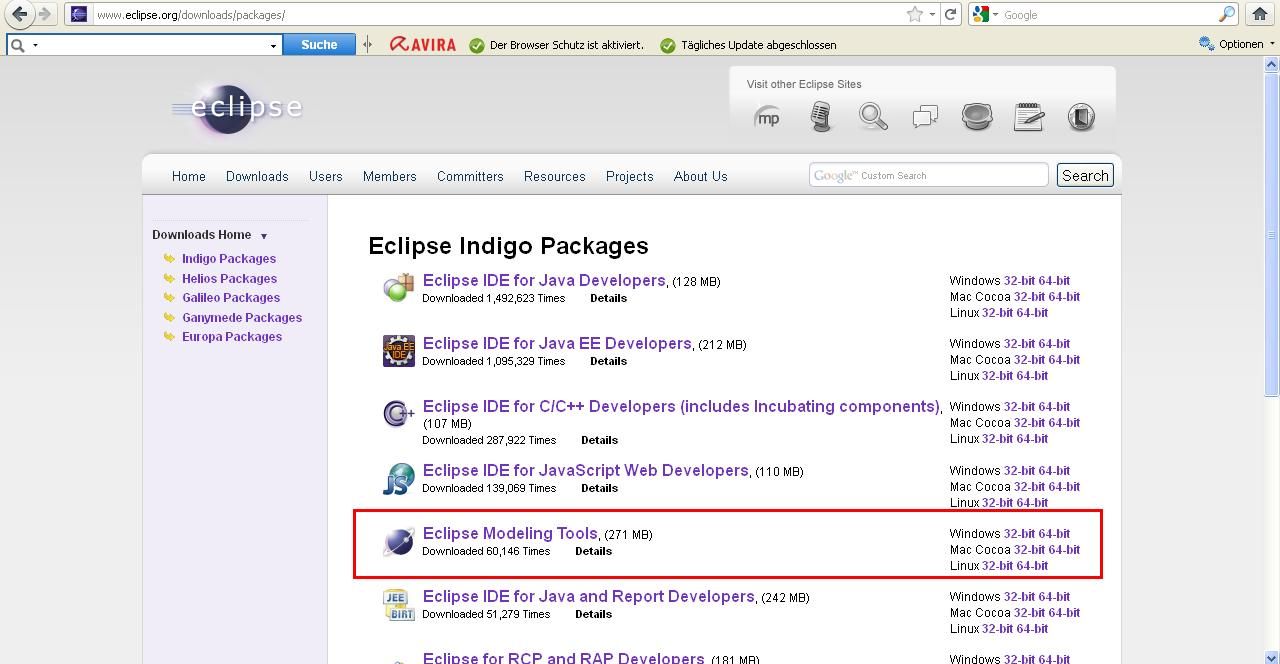
\includegraphics[width=0.5\textwidth]{pics/eclipse_modelingpackage.png}
	\caption{Download Modeling Package}
	\label{fig_downloadModelingPackage}
\end{figure}

%$\blacktriangleright$ Download and install Eclipse.\\
%For a detailed tutorial on how to install Eclipse and Eclipse Plugins please
%refer to http://www.vogella.de/articles/Eclipse/article.html\\
%(Tested for Windows 32bit, 64bit should work as well)\\

$\blacktriangleright$ Start eclipse with a
workspace of your choice.\\

$\blacktriangleright$ Install our Eclipse Plugin.\\
%in eclipse BILD BILD
http://www.moflon.org/fileadmin/download/moflon-ide/eclipse-plugin/update-site2\\
Please note: Calculating requirements and dependencies when installing the
plugin might take quite a while depending on your internet connection! 
You will have to restart Eclipse after installing the plugin.

\section{Step 03: Now, try out our demo}

$\blacktriangleright$ Go to Window/Open Perspective/Other\ldots and choose
Moflon.(Figure \ref{fig_eclipse})\\
\begin{figure}[!h]
	\centering
  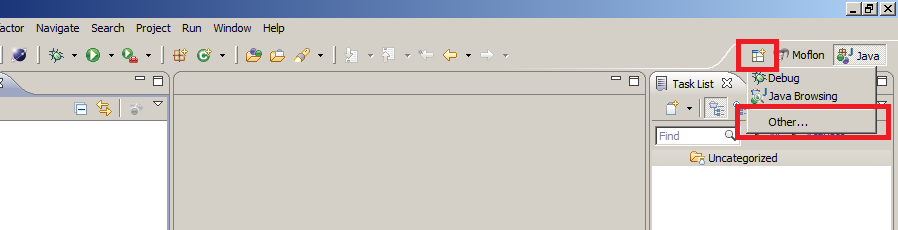
\includegraphics[width=0.5\textwidth]{pics/eclipse_firststart.png}
	\caption{Eclipse}
	\label{fig_eclipse}
\end{figure}
%Bild mit markierung !
%eclipse_firststart.png

$\blacktriangleright$ In the toolbar a new action set should have appeared\ldots
Choose ``New Metamodel''. (Figure \ref{fig_eclipseNewMetamodel})\\
The button with an "L" shows you our logfile (important input for us if
something doesn�t work)\\
\begin{figure}[!h]
	\centering
  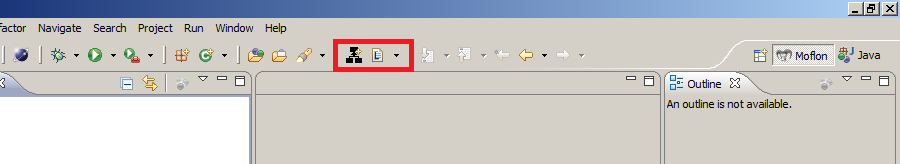
\includegraphics[width=0.8\textwidth]{pics/eclipse_metamodelButton.png}
	\caption{Eclipse New Metamodel}
	\label{fig_eclipseNewMetamodel}
\end{figure}

$\blacktriangleright$ Enter ``demo'' as the name of a new metamodel
project and confirm.\\ 
An empty EA project file ``demo.eap'' will be
created in a new project and working set.\\

$\blacktriangleright$ Choose working sets as your top level element in the
package explorer.(Figure \ref{fig_eclipseWorkingsets})\\
We will work a lot with working sets.\\
%BILD ! eclipse_workingsets.png
\begin{figure}[!h]
	\centering
  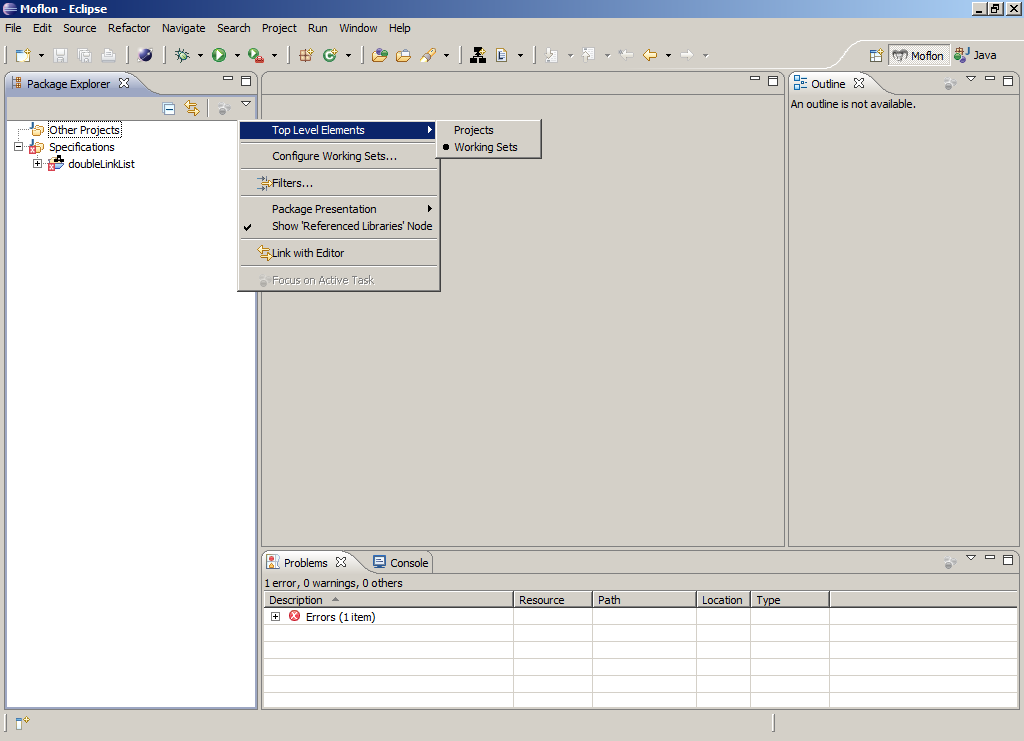
\includegraphics[width=0.5\textwidth]{pics/eclipse_workingsets.png}
	\caption{Eclipse - Working sets}
	\label{fig_eclipseWorkingsets}
\end{figure}

$\blacktriangleright$ Open the newly created project and replace the
``demo.eap'' file with the demo.eap that you will find in the
same folder as this tutorial.\\ 
This EA file already contains our simple demo projects.\\

$\blacktriangleright$ Double click ``demo.eap'' to start EA.
NOTE: Choose ``Ultimate" when starting EA for the first time.\\

$\blacktriangleright$ Choose Add-Ins/MOFLON::Ecore Addin/Export all to Workspace.(Figure \ref{fig_ea})\\
%bild ea_firststart.png
\begin{figure}[!h]
	\centering
  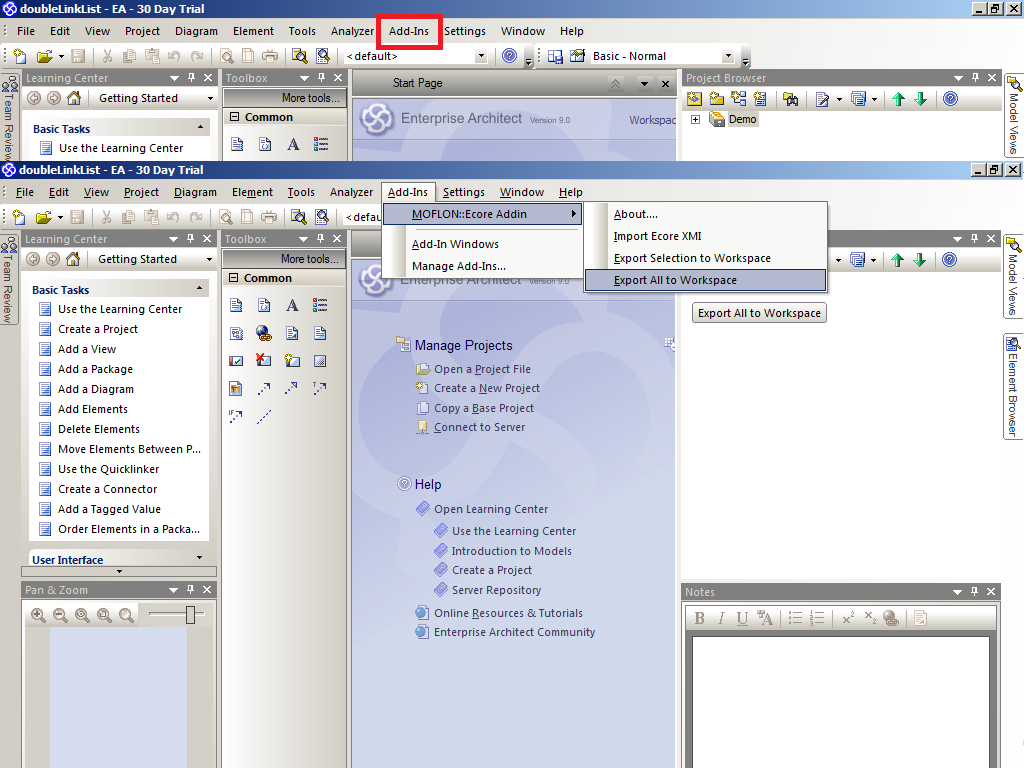
\includegraphics[width=0.6\textwidth]{pics/ea_firststart.png}
	\caption{Enterprise Architect}
	\label{fig_ea}
\end{figure}

$\blacktriangleright$ Switch to Eclipse, choose your Metamodel project and press
F5 (refresh).\\
All projects should be created and the code generator invoked
automatically\ldots\\

\section{Step 04: JUnit tests}

$\blacktriangleright$ Go to ``File - Import - General - Existing Projects
into Workspace'' and import the TestSuite folder.(Figure \ref{fig_eclipseTestsuiteImport})
%bild eclipse_testsuitimport.png
\begin{figure}[!h]
	\centering
  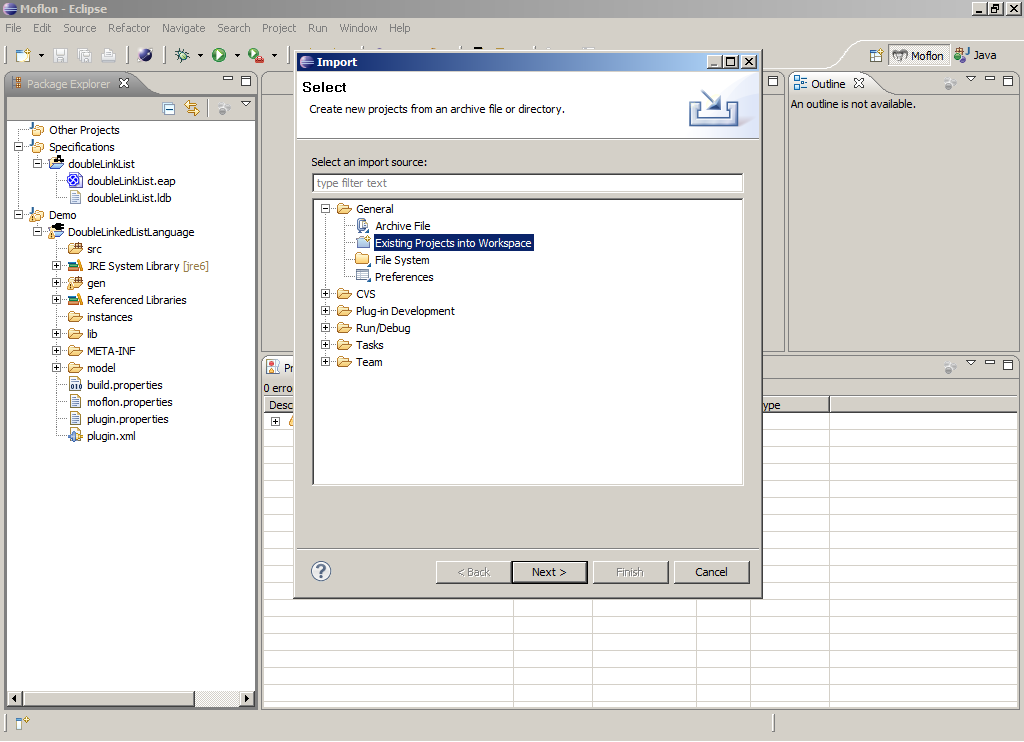
\includegraphics[width=0.6\textwidth]{pics/eclipse_testsuitimport.png}
	\caption{Eclipse Testsuite Import}
	\label{fig_eclipseTestsuiteImport}
\end{figure}

\newpage

The TestSuite should be a project of its own. (Figure \ref{fig_eclipsepackageexplorer})

\begin{figure}[!h]
	\centering
  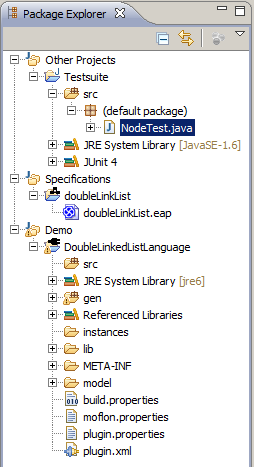
\includegraphics[width=0.2\textwidth]{pics/eclipse_packageexplorer.png}
	\caption{Eclipse Package Explorer}
	\label{fig_eclipsepackageexplorer}
\end{figure}



$\blacktriangleright$ Right-Click on the Testsuite folder - ``Run as'' - ``JUnit
Test''. (Figure \ref{fig_eclipsetestsuiterun})

\begin{figure}[!h]
	\centering
  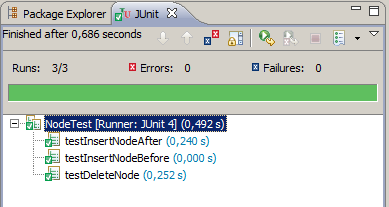
\includegraphics[width=0.2\textwidth]{pics/eclipse_testsuiterun.png}
	\caption{Eclipse TestSuite Run}
	\label{fig_eclipsetestsuiterun}
\end{figure}



\section{Step 05: [Projektstruktur EA]}
\section{Step 06: [Projektstruktur Eclipse]}
